% Options for packages loaded elsewhere
\PassOptionsToPackage{unicode}{hyperref}
\PassOptionsToPackage{hyphens}{url}
%
\documentclass[
  11pt,
]{article}
\usepackage{amsmath,amssymb}
\usepackage{lmodern}
\usepackage{iftex}
\ifPDFTeX
  \usepackage[T1]{fontenc}
  \usepackage[utf8]{inputenc}
  \usepackage{textcomp} % provide euro and other symbols
\else % if luatex or xetex
  \usepackage{unicode-math}
  \defaultfontfeatures{Scale=MatchLowercase}
  \defaultfontfeatures[\rmfamily]{Ligatures=TeX,Scale=1}
\fi
% Use upquote if available, for straight quotes in verbatim environments
\IfFileExists{upquote.sty}{\usepackage{upquote}}{}
\IfFileExists{microtype.sty}{% use microtype if available
  \usepackage[]{microtype}
  \UseMicrotypeSet[protrusion]{basicmath} % disable protrusion for tt fonts
}{}
\makeatletter
\@ifundefined{KOMAClassName}{% if non-KOMA class
  \IfFileExists{parskip.sty}{%
    \usepackage{parskip}
  }{% else
    \setlength{\parindent}{0pt}
    \setlength{\parskip}{6pt plus 2pt minus 1pt}}
}{% if KOMA class
  \KOMAoptions{parskip=half}}
\makeatother
\usepackage{xcolor}
\usepackage[margin=1in]{geometry}
\usepackage{graphicx}
\makeatletter
\def\maxwidth{\ifdim\Gin@nat@width>\linewidth\linewidth\else\Gin@nat@width\fi}
\def\maxheight{\ifdim\Gin@nat@height>\textheight\textheight\else\Gin@nat@height\fi}
\makeatother
% Scale images if necessary, so that they will not overflow the page
% margins by default, and it is still possible to overwrite the defaults
% using explicit options in \includegraphics[width, height, ...]{}
\setkeys{Gin}{width=\maxwidth,height=\maxheight,keepaspectratio}
% Set default figure placement to htbp
\makeatletter
\def\fps@figure{htbp}
\makeatother
\setlength{\emergencystretch}{3em} % prevent overfull lines
\providecommand{\tightlist}{%
  \setlength{\itemsep}{0pt}\setlength{\parskip}{0pt}}
\setcounter{secnumdepth}{-\maxdimen} % remove section numbering
\newlength{\cslhangindent}
\setlength{\cslhangindent}{1.5em}
\newlength{\csllabelwidth}
\setlength{\csllabelwidth}{3em}
\newlength{\cslentryspacingunit} % times entry-spacing
\setlength{\cslentryspacingunit}{\parskip}
\newenvironment{CSLReferences}[2] % #1 hanging-ident, #2 entry spacing
 {% don't indent paragraphs
  \setlength{\parindent}{0pt}
  % turn on hanging indent if param 1 is 1
  \ifodd #1
  \let\oldpar\par
  \def\par{\hangindent=\cslhangindent\oldpar}
  \fi
  % set entry spacing
  \setlength{\parskip}{#2\cslentryspacingunit}
 }%
 {}
\usepackage{calc}
\newcommand{\CSLBlock}[1]{#1\hfill\break}
\newcommand{\CSLLeftMargin}[1]{\parbox[t]{\csllabelwidth}{#1}}
\newcommand{\CSLRightInline}[1]{\parbox[t]{\linewidth - \csllabelwidth}{#1}\break}
\newcommand{\CSLIndent}[1]{\hspace{\cslhangindent}#1}
\usepackage{setspace}\doublespacing
\usepackage{lineno}\linenumbers
\usepackage{booktabs}
\usepackage{longtable}
\usepackage{array}
\usepackage{multirow}
\usepackage{wrapfig}
\usepackage{float}
\usepackage{colortbl}
\usepackage{pdflscape}
\usepackage{tabu}
\usepackage{threeparttable}
\usepackage{threeparttablex}
\usepackage[normalem]{ulem}
\usepackage{makecell}
\usepackage{xcolor}
\ifLuaTeX
  \usepackage{selnolig}  % disable illegal ligatures
\fi
\IfFileExists{bookmark.sty}{\usepackage{bookmark}}{\usepackage{hyperref}}
\IfFileExists{xurl.sty}{\usepackage{xurl}}{} % add URL line breaks if available
\urlstyle{same} % disable monospaced font for URLs
\hypersetup{
  pdftitle={The role of habitat and evolutionary allometry in the morphological differentiation of Pristurus geckos},
  hidelinks,
  pdfcreator={LaTeX via pandoc}}

\title{The role of habitat and evolutionary allometry in the
morphological differentiation of \emph{Pristurus} geckos}
\author{}
\date{\vspace{-2.5em}}

\begin{document}
\maketitle

\begin{center}
\textbf{ORDER TBD:  H{\'{e}}ctor Tejero-Cicu{\'{e}}ndez$^{1,*}$,  Iris Men{\'{e}}ndez$^{2,3}$, Adri{\'{a}} Talavera, Marc Sim{\'{o}}-Riudalbas$^{1}$, Salvador Carranza$^{1}$, and Dean C. Adams$^{4}$}
\end{center}

\begin{center}05 October, 2022\end{center}

\(^{1}\)Institute of Evolutionary Biology (CSIC-Universitat Pompeu
Fabra), Passeig Marítim de la Barceloneta 37-49, Barcelona 08002, Spain

\(^{2}\)Departamento de Geodinámica, Estratigrafía y Paleontología,
Facultad de Ciencias Geológicas, Universidad Complutense de Madrid,
C/José Antonio Novais 12, Madrid 28040, Spain

\(^{3}\)Departamento de Cambio Medioambiental, Instituto de Geociencias
(UCM, CSIC), C/Severo Ochoa 7, Madrid 28040, Spain

\(^{4}\)Department of Ecology, Evolution, and Organismal Biology, Iowa
State University, Ames, Iowa, 50010 USA

\(^{*}\)Correspondence: Héctor Tejero-Cicuéndez
\href{mailto:cicuendez93@gmail.com}{\nolinkurl{cicuendez93@gmail.com}}

\hfill\break

\textbf{Keywords}: Phenotypic Evolution, Morphospace, Allometry,
\emph{Pristurus} geckos \hfill\break

\textbf{Short Title}: XXX \hfill\break

\textbf{Author Contributions}: All authors collaboratively developed the
concept and contributed to all portions of this manuscript. HT-C, IM,
and DCA performed the analyses. All authors approve of the final product
and are willingly accountable for any portion of the
content.\hfill\break

\textbf{Conflicts of Interests}: The authors declare no conflicts of
interest.\hfill\break

\textbf{Data Archiving}: Data are available on DRYAD
(\url{doi:10.5061/dryad.xwdbrv1f6} (Tejero-Cicuéndez et al. 2021b)).
R-scripts are available at \textbf{XXX}. \hfill\break

\textbf{Acknowledgments}: We thank XYZPDQ\ldots{} This work was
sponsored in part by XXX (to SC) DCA was funded in part by National
Science Foundation Grant DBI-1902511.

\newpage

\hypertarget{abstract}{%
\section{Abstract}\label{abstract}}

asdf

\newpage

\hypertarget{introduction}{%
\section{Introduction}\label{introduction}}

Understanding how phenotypic diversity evolves, and elucidating the
forces that generate and maintain this diversity, are major goals in
evolutionary biology. Because adaptive evolution is the product of
natural selection, changes in ecological selection pressures are
expected to affect the evolutionary trajectory of phenotypic traits that
facilitate an organism's survival in their habitat. Evolutionary theory
predicts that differing habitats will exert unique ecological selection
pressures on organisms, resulting in associations between ecological and
phenotypic traits. Indeed, species inhabiting differing habitats often
display functional, behavioral, or phenotypic differences, that have
presumably been the result of adaptive diversification in their
respective ecological habitats (Collar et al. 2010; Kaliontzopoulou et
al. 2015; Price et al. 2015; Martinez et al. 2021; Kolmann et al. 2022).
\hfill\break

One possible evolutionary outcome of ecological specialization is that
organisms inhabiting similar environments display common phenotypic
characteristics. When such patterns occur repeatedly (e.g., Losos 1992;
Schluter and McPhail 1992), this convergent evolution is treated as
strong evidence of adaptation. Indeed the ecomorphological paradigm
(sensu Arnold 1983) is predicated, in part, on such cases, which
emphasize the strong association between the phenotypic traits that
organisms display (morphological, behavioral, or physiological), and the
ecological characteristics of their habitat that mediate organismal
performance. In vertebrates, ecomorphological trends have been well
studied in numerous taxonomic groups, and include the emblematic
`ecomorphs' of Caribbean \emph{Anolis} lizards that exploit different
microhabitats (Losos 1992, 2009; Mahler et al. 2013), differential beak
morphology in species of Darwin's finches (Schluter and Grant 1984;
Grant and Grant 2006; Reaney et al. 2020), the recurring phenotypes of
African lake cichlids across ecological regimes (Albertson and Kocher
2001; Urban et al. 2022), and the distinct body forms of freshwater
fishes in benthis and limnetic habitats (Jastrebski and Robinson 2004;
Berner et al. 2008; Stuart et al. 2017) among others. \hfill\break

However, while the patterns of morphological differences in distinct
ecological contexts have been well documented, less-well understood is
how this differentiation has been influenced by the covariance between
body parts resulting from body size variation (i.e., allometry). It has
long been recognized that the interrelationships among traits can have a
strong influence on how phenotypic evolution proceeds, as trait
correlations influence the degree to which phenotypic variation is
exposed to selection (Wagner and Altenberg 1996). Thus, the integration
among traits can constrain phenotypic change in certain directions, or
enhance variation along other phenotypic axes (Schluter 1996; Wagner and
Altenberg 1996; Wagner and Zhang 2011; Klingenberg and Marugán-Lobón
2013; Goswami et al. 2014, 2016; Felice et al. 2018). Further, because
nearly all linear traits covary strongly with overall body size
(Jolicoeur 1963; Bookstein 2022), allometric trends could be considered
the quintessential measure of phenotypic integration. Thus, identifying
whether allometric patterns differ across habitats, and how such
patterns of trait covariation affect ecomorphological trends among
species utilizing those habitats, remains an important question worthy
of investigation. \hfill\break

The Afro-Arabian geckos in the genus \emph{Pristurus} afford the
opportunity to elucidate the interdigitating effects of allometry and
habitat specialization on clade-level patterns of phenotypic diversity.
Prior work on this system (Tejero-Cicuéndez et al. 2021a) revealed that
the colonization of ground habitats has been a trigger of morphological
change, specifically reflected in an increase in body size and shape
disparity. Interestingly, some ground-dwelling species are among the
largest of the genus and also show increased relative head sizes and
limb proportions, while some other species with this ecological
specialization have evolved to be among the smallest of the group.
Additionally, among the species exploiting rocky habitats (the most
common ecological feature in \emph{Pristurus}), there are also species
with both considerably large and small body sizes (Tejero-Cicuéndez et
al. 2021a). What remains unexplored, however, is how the evolution of
body shape is related to differences in body size and whether habitat
specialization has an impact in this shape-size relationship.
\hfill\break

In this study, we employed a combination of multivariate morphometric
and phylogenetic comparative analysis to interrogate macroevolutionary
patterns of evolutionary allometry in \emph{Pristurus} geckos of
Afro-Arabia. Using phenotypic, phylogenetic, and ecological data, we
first characterized allometric trends in body form in the group, to
discern the extent to which allometric patterns differed across species
occupying distinct ecological habitats. We then examined changes in
allometric trends across the phylogeny, and linked these patterns to
overall phenotypic integration, diversification in morphospace, and
habitat utilization among taxa. Overall our results demonstrate that the
interplay between ecological specialization and differing allometric
trajectories in species with disparate body size may have a determinant
role in shaping the phenotypic evolution and hence in adaptive dynamics
in this clade.

\hypertarget{materials-and-methods}{%
\section{Materials and Methods}\label{materials-and-methods}}

\hypertarget{data}{%
\subsection{Data}\label{data}}

We used a combination of phenotypic, phylogenetic, and ecological data
to characterize and evaluate intra- and interspecific allometric trends.
The data utilized here were obtained from our prior work on this system
(Tejero-Cicuéndez et al. 2021a, 2022), and are briefly described here.
First we used a time-dated, molecular phylogeny that included all
members of the genus \emph{Pristurus}, including several currently
undescribed taxa. The tree was estimated in a Bayesian framework, using
five mitochondrial markers, six nuclear markers, and 21 calibration
points (for details see Tejero-Cicuéndez et al. 2022). Next we
categorized each species as belonging to one of three ecological groups
(ground, rock, or tree), based on descriptions of habitat use found in
the literature (see Tejero-Cicuéndez et al. 2021a). Finally, we obtained
a phenotypic data set containing body size (snout-vent length: SVL) and
eight linear measurements (Figure 1) that described overall body form:
trunk length (TrL), head length (HL), head width (HW), head height (HH),
humerus length (Lhu), ulna length (Lun), femur length (Lfe), and tibia
length (Ltb) (Tejero-Cicuéndez et al. 2021a). We restricted our study to
those species represented by nine or more individuals; resulting in a
dataset of 687 individuals from 25 species (invidivuals per species:
\(\mu=27\); min = 9, max = 56). Species in the phenotypic dataset were
then matched to the phylogeny, which was subsequently pruned to arrive
at the final topology. All measurements were log-transformed prior to
statistical analyses. Additional details regarding data collection and
formal descriptions of each linear measurement may be found in the
original sources (see Tejero-Cicuéndez et al. 2021a, 2022). The data are
found on DRYAD: \url{https://doi.org/10.5061/dryad.xwdbrv1f6}
(Tejero-Cicuéndez et al. 2021b).

\hypertarget{statistical-and-comparative-analyses}{%
\subsection{Statistical and Comparative
Analyses}\label{statistical-and-comparative-analyses}}

We conducted a series of analyses to interrogate allometric trends,
patterns of integration, and macroevolutionary changes in allometry,
relative to differentiation in body form. First we characterized
evolutionary allometry in the genus by performing a phylogenetic
multivariate regression of body form on size, using the species means as
data. We then performed an analogous procedure at the individual level,
regressing body form on size using our entire dataset. From both the
species-level (phylogenetic) and the individual-level regression models,
we obtained the set of regression coefficients, and calculated the
difference between them to describe the extent to which patterns of
allometry at the individual level were concordant with evolutionary
allometric trends across species. \hfill\break

Next we used the individual dataset to determine whether allometric
trends in body form differed across habitat groups. This was
accomplished by performing a multivariate analysis of covariance, with
body size (\(SVL\)), \(habitat\), and \(SVL\times habitat\) as model
effects. Significance was evaluated using 999 iterations of a
permutation procedure, where residuals from a reduced model were
randomly permuted in each permutation (RRPP), model statistics were
recalculated, and used to generate empirical null sampling distributions
to evaluate the observed test statistics (following Freedman and Lane
1983; Collyer and Adams 2007; Collyer et al. 2015). We then compared the
multivariate allometric vectors for each habitat group by calculating
pairwise differences in their angular direction in morphospace, and
evaluating these relative to empirical sampling distributions obtained
through RRPP (Collyer and Adams 2007; Adams and Collyer 2009; Collyer
and Adams 2013). Patterns of multivariate allometry relative to body
size were visualized via regression scores (Drake and Klingenberg 2008)
and predicted lines (Adams and Nistri 2010), based on the coefficients
and fitted values from the linear model described above. \hfill\break

We then examined changes in allometric trends across the phylogeny. Here
we treated the head dimensions and limb dimensions separately, as
allometric trends could potentially differ between these body regions
due to differential functional or selective constraints (Kaliontzopoulou
et al. 2010). Because both the head and limb data were multivariate, we
first performed a partial least squares analysis (Rohlf and Corti 2000)
of the head traits versus SVL, and the limb traits versus SVL, to
describe the direction of maximal covaration between each body region
and size. PLS scores from each analysis were obtained, and
species-specific slopes describing the extent of head and limb allometry
within each species were extracted from an analysis of covariance
modeled as: \(PLS1_{head} \sim SVL*species\) and
\(PLS1_{limb} \sim SVL*species\) respectively. The species-specific
allometric slopes were then mapped on the phylogeny of \emph{Pristurus}
using a Brownian motion model of evolution, to qualitatively evaluate
shifts in allometry across the phylogeny for the group (for a similar
approach see Adams and Nistri 2010). \hfill\break

Next, because allometry describes the extent to which traits covary with
size and with each other (i.e., integration), we conducted an analysis
of integration. Here we characterized the extent of morphological
integration in body form for individuals within each habitat group.
Integration was estimated using the relative eigenvalue variance
(\(V_{rel}\): Pavlicev et al. 2009), which summarizes the dispersion of
eigenvalues of the trait covariance matrix (see Conaway and Adams 2022).
To compare the strength of morphological integration across habitat
groups, we converted \(V_{rel}\) to an effect size (\(Z\)-score) which
measures the strength of integration (Conaway and Adams 2022), and
performed a series of two-sample tests to compare effect sizes among
habitat groups. Additionally and for comparison, we repeated these
analyses on the set of size-standardized trait data, found as a set of
shape ratios (sensu Mosimann 1970) where each trait was divided by body
size (Supplemental Information). \hfill\break 

Finally, to relate within-species allometric trends with patterns of
phenotypic diversification in the group we generated a phylomorphospace,
based on the size-standardized species means obtained from a
phylogenetic regression (see Tejero-Cicuéndez et al. 2021a). Here,
phenotypic similarities among species, relative to their phylogenetic
relationships and habitat affiliations, were observed. All analyses were
conducted in R 4.2.1 (R Core Team 2022), using \texttt{RRPP} version
1.3.1 (Collyer and Adams 2018; Collyer and Adams 2022) and
\texttt{geomorph} 4.0.4 (Baken et al. 2021), and scripts written by the
authors (available at \textbf{XXX}).

\hypertarget{results}{%
\section{Results}\label{results}}

Using phylogenetic regression, we found significant evolutionary
allometry in body form across species (\(N_{sp}=25\); \(F = 217.9\);
\(Z =5.53\); \(P < 0.001\)). Likewise, when allometry in body form was
examined across individuals, a similar pattern was observed
(\(N_{ind}=687\); \(F = 7910.8\); \(Z =9.20\); \(P < 0.001\)). Further,
the vectors of regression coefficients between the two analyses were
highly correlated (\(\rho = 0.94\)) and were oriented in nearly parallel
directions in morphospace (\(\theta = 1.49^\circ\)). This revealed that
the pattern of multivariate allometry across individuals was concordant
with macroevolutionary trends of interspecific allometry among species
of \emph{Pristurus} across the phylogeny. \hfill\break

Our analyses also exposed significant differences in the allometry of
body form among \emph{Pristurus} utilizing distinct habitats (Table 1).
Here, comparisons of multivariate allometric vectors identified that
ground-dwelling \emph{Pristurus} displayed a distinct allometric trend
as compared with \emph{Pristurus} occupying both the rock and tree
habitats (Table 2). In addition, allometric patterns in both rock and
tree habitats were similar to the multivariate line of isometry (Figure
2), while patterns of multivariate allometry in ground-dwelling
\emph{Pristurus} was decidely steeper. Inspection of the regression
coefficients for each trait (Supplemental Information) confirmed the
steeper allometric coefficients for all head and limb traits in
ground-dwelling \emph{Pristurus} as compared with rock and tree-dwelling
taxa, corroborating this result. Taken together, these findings implied
that larger individuals of ground-dwelling \emph{Pristurus} species
displayed proportionately larger heads and limbs, as compared with large
individuals in taxa utilizing other habitat types. A visualization of
multivariate allometric trends (Figure 2) confirmed these statistical
findings, and indicated that the allometric trajectory in
ground-dwelling animals was more extreme as compared with either rock or
tree-dwelling \emph{Pristurus}. \hfill\break

Examination of patterns of trait covariation revealed strong levels of
morphological integration within each habitat type (\(Z_{ground}=3.97\);
\(Z_{rock}=3.72\); \(Z_{tree}=2.15\)). Further, two-sample tests
revealed that the strength of morphological integration was
significantly greater in ground-dwelling \emph{Pristurus} than either
those utilizing rock (\(Z_{Groung-Rock}=6.59\); \(P << 0.001\)) or tree
habitats (\(Z_{Groung-Tree}=11.17\); \(P << 0.001\)). \emph{Pristurus}
utilizing tree habitats displayed the lowest levels of integration,
which were also significantly less than in the rock habitat
(\(Z_{Rock-Tree}=7.19\); \(P << 0.001\)). When size was accounted for in
the data, levels of integration dropped considerably, though the overall
pattern and differences among habitat groups remained the same
(Supplemental Information). \hfill\break

When allometric patterns were mapped on the phylogeny, traitgrams
elucidated that changes in allometric trends were not concentrated to
specific regions of the phylogeny (Figure 3). Rather, increases and
decreases in allometry of both the head traits and the limb traits
occurred repeatedly (see also Supplemental Information). When these
patterns were viewed relative to body size, large ground-dwelling
species tended to display steeper head allometry as compared to large
rock-dwelling species, who displayed shallower head allometry (Figure
3A). Likewise, a similar pattern was observed when comparing small
species utilizing these habitats. In contrast, large ground-dwelling
species exhibited intermediate patterns of limb allometry, and small
species in general were more variable in such patterns (Figure 3B).
Inspection of traitgrams thus revealed some degree of discordance in
patterns of allometry across body regions; a pattern evidenced by the
relatively low correlation between slopes representing head and limb
allometry respectively (\(\rho = 0.42\)). \hfill\break

Finally, when body shape differentiation in \emph{Pristurus} was viewed
in phylomorphospace (Figure 4), we found broad overlap among habitat
groups, though arboreal (tree-dwelling) species were somewhat more
separated in morphospace. Rock-dwelling species occupied a slightly
larger region of morphospace as compared with the other groups, though
this pattern was not statistically significant (Supplemental
Information). Intriguingly, when viewed in relation to body size, large
\emph{Pristurus} species were not localized to a particular region of
morphospace, nor were smaller species. Instead, the largest
rock-dwelling species were found in close proximity to the smallest
ground-dwelling species, indicating that they were similar in overall
body shape. Likewise, the smaller rock-dwelling species were found close
to large ground-dwelling species in morphospace, indicating they
displayed similar body shapes as well. Thus, synthesizing the patterns
revealed in the phylomorphospace with those identified in our earlier
analyses revealed a complex interplay between body shape, body size,
habitat use, morphological integration, and multivariate allometry;
where species with similar body shapes displayed differing overall size,
were found in distinct habitats, and exhibited different allometric
trends.

\hypertarget{discussion}{%
\section{Discussion}\label{discussion}}

\begin{itemize}
\item
  First paragraph; restate topic/questions (see last par of Intro);
  summarize general findings \ldots{}

  \begin{itemize}
  \tightlist
  \item
    something about linking allometry and phenotypic diversification?
  \end{itemize}
\item
  result 1: allometry; overall trend among species nearly identical to
  that among individuals. Thus, patterns of static and evolutionary
  allometry are consistent in \emph{Pristurus}\ldots{} Something else
  about this
\item
  result 2: Allometry differs among habitat groups: `steeper' allometry
  in Ground-dwelling (implication: proportionately larger heads and
  longer limbs in species at larger body sizes).
\item
  result 3: Morphological integration differs among habitat groups.
  Strongest in ground-dwelling; weakest in tree-dwelling. SOME MEANING
  (combined with allometric trend implies that patterns of trait
  covariation are more constrained within ground-dwelling\ldots. Thus,
  differences in body form are most likely found along this primary
  axis\ldots{} (harken to Schluter evolution along lines of least
  resistance)

  \begin{itemize}
  \tightlist
  \item
    Additionally, rank-order of magnitude of integration across habitat
    groups corresponds with the range of body sizes in each:
    ground-dwelling display the largest size-range, while tree-dwelling
    the least (Supp. Information). On the one hand this matches the
    expectation that much of the integration observed in
    \emph{Pristurus} is the result of allometric trends\ldots. And the
    fact that levels of integration drop so precipitously when data are
    size-standardized are in accord with this interpretation.
    Nevertheless, when size is accounted for, the rank-order of
    magnitudes of integration remain the same, implying that
    ground-dwelling \emph{Pristurus} are still relatively constrained in
    patterns of trait covariation as compared with the other two groups.
  \end{itemize}
\item
  result 4: morphospace: Thus there was a reciprocal relationship
  between body shape and body size across ground-dwelling and
  rock-dwelling species. SOMEHOW TIE THIS TO integration (DCA pondering
  this one)
\item
  one interesting\ldots{} head vs.~(correlation of head vs.~limb slopes:
  0.42. Pretty low. Implies some sort of differential something here,
  resulting in distinct allometric patterns for these two body regions.
  SImilar to Antigoni's work (and refs therein). IMPLICATION: tie this
  into integration/modularity. Less integrated across the whole
  organism, and more modular\ldots{} Future studies should examine this.
\end{itemize}

In conclusion\ldots{} paragraph

\newpage

\hypertarget{references}{%
\section*{References}\label{references}}
\addcontentsline{toc}{section}{References}

\setlength{\parindent}{-0.25in} \setlength{\leftskip}{0.25in}
\setlength{\parskip}{8pt} \noindent

\hypertarget{refs}{}
\begin{CSLReferences}{1}{0}
\leavevmode\vadjust pre{\hypertarget{ref-AdamsCollyer2009}{}}%
Adams, D. C., and M. L. Collyer. 2009. A general framework for the
analysis of phenotypic trajectories in evolutionary studies. Evolution
63:1143--1154.

\leavevmode\vadjust pre{\hypertarget{ref-AdamsNistri2010}{}}%
Adams, D. C., and A. Nistri. 2010. Ontogenetic convergence and evolution
of foot morphology in european cave salamanders (family:
plethodontidae). BMC Evolutionary Biology 10:1--10. BioMed Central.

\leavevmode\vadjust pre{\hypertarget{ref-Albertson2001}{}}%
Albertson, R. C., and T. D. Kocher. 2001. Assessing morphological
differences in an adaptive trait: A landmark-based morphometric
approach. Journal of Experimental Zoology 289:385--403.

\leavevmode\vadjust pre{\hypertarget{ref-Arnold1983}{}}%
Arnold, S. J. 1983. Morphology, performance, fitness. American Zoologist
23:347--361.

\leavevmode\vadjust pre{\hypertarget{ref-Baken2021}{}}%
Baken, E. K., M. L. Collyer, A. Kaliontzopoulou, and D. C. Adams. 2021.
Geomorph 4.0 and gmShiny: Enhanced analytics and a new graphical
interface for a comprehensive morphometric experience. Methods in
Ecology and Evolution 12:2355--2363.

\leavevmode\vadjust pre{\hypertarget{ref-BERNER2008}{}}%
Berner, D., D. C. Adams, A.-C. Grandchamp, and A. P. Hendry. 2008.
Natural selection drives patterns of lake-stream divergence in
stickleback foraging morphology. Journal of Evolutionary Biology
21:1653--1665.

\leavevmode\vadjust pre{\hypertarget{ref-Bookstein2022}{}}%
Bookstein, F. L. 2022. Dimensions of morphological integration.
Evolutionary Biology 49:342--372.

\leavevmode\vadjust pre{\hypertarget{ref-COLLAR2010}{}}%
Collar, D. C., J. A. Schulte, B. C. O'Meara, and J. B. Losos. 2010.
Habitat use affects morphological diversification in dragon lizards.
Journal of Evolutionary Biology 23:1033--1049.

\leavevmode\vadjust pre{\hypertarget{ref-CollyerAdams2007}{}}%
Collyer, M. L., and D. C. Adams. 2007. Analysis of two-state
multivariate phenotypic change in ecological studies. Ecology
88:683--692.

\leavevmode\vadjust pre{\hypertarget{ref-CollyerAdams2013}{}}%
Collyer, M. L., and D. C. Adams. 2013. Phenotypic trajectory analysis:
Comparison of shape change patterns in evolution and ecology. Hystrix
24:75--83.

\leavevmode\vadjust pre{\hypertarget{ref-RRPP}{}}%
Collyer, M. L., and D. C. Adams. 2022.
\href{https://CRAN.R-project.org/package=RRPP}{R: RRPP: Linear model
evaluation with randomized residuals in a permutation procedure. Vsn.
1.3.1}. R Foundation for Statistical Computing, Vienna, Austria.

\leavevmode\vadjust pre{\hypertarget{ref-CollyerAdams2018}{}}%
Collyer, M. L., and D. C. Adams. 2018. RRPP: An r package for fitting
linear models to high-dimensional data using residual randomization.
Methods in Ecology and Evolution 9:1772--1779.

\leavevmode\vadjust pre{\hypertarget{ref-Collyer_et_al2015}{}}%
Collyer, M. L., D. J. Sekora, and D. C. Adams. 2015. A method for
analysis of phenotypic change for phenotypes described by
high-dimensional data. Heredity 115:357--365.

\leavevmode\vadjust pre{\hypertarget{ref-ConawayAdams2022}{}}%
Conaway, M. A., and D. C. Adams. 2022.
\href{https://doi.org/10.1111/evo.14595}{An effect size for comparing
the strength of morphological integration across studies}. Evolution
76:(In Press).

\leavevmode\vadjust pre{\hypertarget{ref-DrakeKlingenberg2008}{}}%
Drake, A. G., and C. P. Klingenberg. 2008.
\href{https://doi.org/10.1098/rspb.2007.1169}{The pace of morphological
change: Historical transformation of skull shape in st bernard dogs}.
Proceedings of the Royal Society B: Biological Sciences 275:71--76.

\leavevmode\vadjust pre{\hypertarget{ref-Felice2018}{}}%
Felice, R. N., M. Randau, and A. Goswami. 2018. A fly in a tube:
Macroevolutionary expectations for integrated phenotypes. Evolution
72:2580--2594.

\leavevmode\vadjust pre{\hypertarget{ref-Freedman1983}{}}%
Freedman, D., and D. Lane. 1983. A nonstochastic interpretation of
reported significance levels. Journal of Business {\&} Economic
Statistics 1:292--298.

\leavevmode\vadjust pre{\hypertarget{ref-Goswami2016}{}}%
Goswami, A., M. Randau, P. D. Polly, V. Weisbecker, C. Verity Bennett,
L. Hautier, and M. R. Sánchez-Villagra. 2016.
\href{https://doi.org/10.1093/icb/icw039}{Do developmental constraints
and high integration limit the evolution of the marsupial oral
apparatus?} Integrative and Comparative Biology 56:404--415.

\leavevmode\vadjust pre{\hypertarget{ref-Goswami2014}{}}%
Goswami, A., J. B. Smaers, C. Soligo, and P. D. Polly. 2014.
\href{https://doi.org/10.1098/rstb.2013.0254}{The macroevolutionary
consequences of phenotypic integration: From development to deep time}.
Philosophical Transactions of the Royal Society B: Biological Sciences
369:20130254.

\leavevmode\vadjust pre{\hypertarget{ref-Grant2006}{}}%
Grant, P. R., and B. R. Grant. 2006. Evolution of character displacement
in darwin's finches. Science 313:224--226.

\leavevmode\vadjust pre{\hypertarget{ref-Jastrebski2004}{}}%
Jastrebski, C. J., and B. W. Robinson. 2004. Natural selection and the
evolution of replicated trophic polymorphisms in pumpkinseed sunfish
(\emph{{L}epomis gibbosus}). Evolutionary Ecology Research 6:285--305.

\leavevmode\vadjust pre{\hypertarget{ref-Jolicoeur1963}{}}%
Jolicoeur, P. 1963. The multivariate generalization of the allometry
equation. Biometrics 19:497--499.

\leavevmode\vadjust pre{\hypertarget{ref-Kaliontzopoulou2015}{}}%
Kaliontzopoulou, A., M. A. Carretero, and D. C. Adams. 2015.
Ecomorphological variation in male and female wall lizards and the
macroevolution of sexual dimorphism in relation to habitat use. Journal
of Evolutionary Biology 28:80--94.

\leavevmode\vadjust pre{\hypertarget{ref-KALIONTZOPOULOU2010}{}}%
Kaliontzopoulou, A., M. A. Carretero, and G. A. Llorente. 2010.
Intraspecific ecomorphological variation: Linear and geometric
morphometrics reveal habitat-related patterns within \emph{{P}odarcis
bocagei} wall lizards. Journal of Evolutionary Biology 23:1234--1244.

\leavevmode\vadjust pre{\hypertarget{ref-Klingenberg2013}{}}%
Klingenberg, C. P., and J. Marugán-Lobón. 2013. Evolutionary covariation
in geometric morphometric data: Analyzing integration, modularity, and
allometry in a phylogenetic context. Systematic Biology 62:591--610.

\leavevmode\vadjust pre{\hypertarget{ref-Kolmann2022}{}}%
Kolmann, M. A., F. P. L. Marques, J. C. Weaver, M. N. Dean, J. P.
Fontenelle, and N. R. Lovejoy. 2022. Ecological and phenotypic
diversification after a continental invasion in neotropical freshwater
stingrays. Integrative and Comparative Biology 62:424--440.

\leavevmode\vadjust pre{\hypertarget{ref-Losos2009}{}}%
Losos, J. B. 2009. Lizards in an evolutionary tree: Ecology and adaptive
radiation of anoles. University of California Press.

\leavevmode\vadjust pre{\hypertarget{ref-Losos1992}{}}%
Losos, J. B. 1992. The evolution of convergent structure in {C}aribbean
\emph{{A}nolis} communities. Systematic Biology 41:403--420.

\leavevmode\vadjust pre{\hypertarget{ref-Mahler2013}{}}%
Mahler, D. L., T. Ingram, L. J. Revell, and J. B. Losos. 2013.
Exceptional convergence on the macroevolutionary landscape in island
lizard radiations. Science 341:292--295.

\leavevmode\vadjust pre{\hypertarget{ref-Martinez2021}{}}%
Martinez, C. M., S. T. Friedman, K. A. Corn, O. Larouche, S. A. Price,
and P. C. Wainwright. 2021. The deep sea is a hot spot of fish body
shape evolution. Ecology Letters 24:1788--1799.

\leavevmode\vadjust pre{\hypertarget{ref-Mosimann1970}{}}%
Mosimann, J. E. 1970. Size allometry: Size and shape variables with
characterizations of the lognormal and generalized gamma distributions.
Journal of the American Statistical Association 65:930--945.

\leavevmode\vadjust pre{\hypertarget{ref-Pavlicev2009}{}}%
Pavlicev, M., J. M. Cheverud, and G. P. Wagner. 2009.
\href{https://doi.org/10.1007/s11692-008-9042-7}{Measuring morphological
integration using eigenvalue variance}. Evolutionary Biology
36:157--170.

\leavevmode\vadjust pre{\hypertarget{ref-Price2015}{}}%
Price, S. A., S. T. Friedman, and P. C. Wainwright. 2015. How predation
shaped fish: The impact of fin spines on body form evolution across
teleosts. Proceedings of the Royal Society B: Biological Sciences
282:20151428.

\leavevmode\vadjust pre{\hypertarget{ref-RCT}{}}%
R Core Team. 2022. \href{https://www.R-project.org/}{R: A language and
environment for statistical computing. Version 4.2.1}. R Foundation for
Statistical Computing, Vienna, Austria.

\leavevmode\vadjust pre{\hypertarget{ref-Reaney2020}{}}%
Reaney, A. M., Y. Bouchenak-Khelladi, J. A. Tobias, and A. Abzhanov.
2020. Ecological and morphological determinants of evolutionary
diversification in darwin{\textquotesingle}s finches and their
relatives. Ecology and Evolution 10:14020--14032.

\leavevmode\vadjust pre{\hypertarget{ref-Rohlf2000}{}}%
Rohlf, F. J., and M. Corti. 2000. Use of two-block partial least-squares
to study covariation in shape. Systematic Biology 49:740--753.

\leavevmode\vadjust pre{\hypertarget{ref-Schluter1996}{}}%
Schluter, D. 1996. Adaptive radiation along genetic lines of least
resistance. Evolution 50:1766--1774.

\leavevmode\vadjust pre{\hypertarget{ref-Schluter1984}{}}%
Schluter, D., and P. R. Grant. 1984. Determinants of morphological
patterns in communities of darwin{\textquotesingle}s finches. The
American Naturalist 123:175--196.

\leavevmode\vadjust pre{\hypertarget{ref-Schluter1992}{}}%
Schluter, D., and J. D. McPhail. 1992. Ecological character displacement
and speciation in sticklebacks. The American Naturalist 140:85--108.

\leavevmode\vadjust pre{\hypertarget{ref-Stuart2017}{}}%
Stuart, Y. E., T. Veen, J. N. Weber, D. Hanson, M. Ravinet, B. K.
Lohman, C. J. Thompson, T. Tasneem, A. Doggett, R. Izen, N. Ahmed, R. D.
H. Barrett, A. P. Hendry, C. L. Peichel, and D. I. Bolnick. 2017.
Contrasting effects of environment and genetics generate a continuum of
parallel evolution. Nature Ecology and Evolution 1:158.

\leavevmode\vadjust pre{\hypertarget{ref-Tejero-Cicuendez2022}{}}%
Tejero-Cicuéndez, H., A. H. Patton, D. S. Caetano, J. Šmíd, L. J.
Harmon, and S. Carranza. 2022. Reconstructing squamate biogeography in
afro-arabia reveals the influence of a complex and dynamic geologic
past. Systematic Biology 71:261--272.

\leavevmode\vadjust pre{\hypertarget{ref-Tejero-Cicuendez2021}{}}%
Tejero-Cicuéndez, H., M. Simó-Riudalbas, I. Menéndez, and S. Carranza.
2021a. \href{https://doi.org/10.1098/rspb.2021.1821}{Ecological
specialization, rather than the island effect, explains morphological
diversification in an ancient radiation of geckos}. Proceedings of the
Royal Society B: Biological Sciences 288:20211821.

\leavevmode\vadjust pre{\hypertarget{ref-PristurusData}{}}%
Tejero-Cicuéndez, H., M. Simó-Riudalbas, I. Menéndez, and S. Carranza.
2021b. Ecological specialization, rather than the island effect,
explains morphological diversification in an ancient radiation of
geckos. Dryad digital repository. (Doi:10.5061/dryad.xwdbrv1f6).

\leavevmode\vadjust pre{\hypertarget{ref-Urban2022}{}}%
Urban, S., J. Gerwin, C. D. Hulsey, A. Meyer, and C. F. Kratochwil.
2022. The repeated evolution of stripe patterns is correlated with body
morphology in the adaptive radiations of east african cichlid fishes.
Ecology and Evolution 12:e8568.

\leavevmode\vadjust pre{\hypertarget{ref-Wagner2011}{}}%
Wagner, G. P., and J. Zhang. 2011. The pleiotropic structure of the
genotype{\textendash}phenotype map: The evolvability of complex
organisms. Nature Reviews Genetics 12:204--213.

\leavevmode\vadjust pre{\hypertarget{ref-Wagner1996}{}}%
Wagner, G., and L. Altenberg. 1996. Perspective: Complex adaptations and
the evolution of evolvability. Evolution 50:967--976.

\end{CSLReferences}

\newpage

\begin{table}[H]

\caption{\label{tab:unnamed-chunk-1}Multivariate analysis of covariance describing variation in body form in \textit{Pristurus}.}
\centering
\begin{tabular}[t]{llllllll}
\toprule
  & Df & SS & MS & Rsq & F & Z & Pr(>F)\\
\midrule
svl & 1 & 516.036559 & 516.0365588 & 0.9203096 & 10188.69842 & 9.490057 & 0.001\\
habitat & 2 & 6.218510 & 3.1092552 & 0.0110902 & 61.38957 & 9.322480 & 0.001\\
svl:habitat & 2 & 3.974307 & 1.9871536 & 0.0070879 & 39.23464 & 7.077264 & 0.001\\
Residuals & 681 & 34.491245 & 0.0506479 & 0.0615124 &  &  & \\
Total & 686 & 560.720622 &  &  &  &  & \\
\bottomrule
\end{tabular}
\end{table}

\newpage

\begin{table}[H]

\caption{\label{tab:unnamed-chunk-2}Pairwise comparisons of multivariate allometry vectors. Effect sizes ($Z_{\theta_{12}}$) based on pairwise differences in angular direction are below the diagonal, and their corresponding significance levels are above diagonal. Significant values in bold.}
\centering
\begin{tabular}[t]{llll}
\toprule
  & Ground & Rock & Tree\\
\midrule
Ground & 0 & \textbf{0.001} & \textbf{0.001}\\
Rock & \textbf{6.872} & 0 & 0.261\\
Tree & \textbf{3.657} & 0.649 & 0\\
\bottomrule
\end{tabular}
\end{table}

\newpage

\hypertarget{figures}{%
\section{Figures}\label{figures}}

Figure 1. Linear Measurements used in this study. SVL = snout-vent
length, TL = trunk length, HL = head length, HW = head width, HH = head
height, Lhu = humerus length, Lun = ulna length, Lfe = femur length, Ltb
= tibia length (for details see Tejero-Cicuéndez et al. 2021a).
\hfill\break

Figure 2. Plot of regression scores and predicted lines representing the
relationship between linear body measurements and size (SVL).
Individuals are colored by habitat use: ground (beige), rock (dark
purple), and tree (magenta). Isometric trend represented by the dashed
line. \hfill\break

Figure 3. Traitgrams showing the evolution of body size (SVL) through
time based on the phylogenetic tree of \emph{Pristurus}. Colors
represent an evolutionary mapping of regression slopes describing the
relationship of (A) head morphology versus body size, and (B) limb
proportions versus body size (see text for descriptions). Species names
are colored by habitat use: ground (beige), rock (dark purple), and tree
(magenta). \hfill\break

Figure 4. Phylomorphospace of \emph{Pristurus}, based on residuals from
a phylogenetic regression of body measurements on size (SVL). Species
means are colored by habitat use: ground (beige), rock (dark purple),
and tree (magenta). Large and small rock-dwelling and ground-dwelling
are highlighted with darker colors to highlight their differentiation
and relative positions in morphospace.

\newpage

\begin{figure}

{\centering 
\includegraphics[width=1\linewidth]{Figs/Fig1} 

}

\caption{Linear Measurements used in this study. SVL = snout-vent length, TL = trunk length, HL = head length, HW = head width, HH = head height, Lhu = humerus length, Lun = ulna length, Lfe = femur length, Ltb = tibia length (for details see Tejero-Cicu{'{e}}ndez et al. 2021a).}\label{fig:unnamed-chunk-3}
\end{figure}

\newpage

\begin{figure}
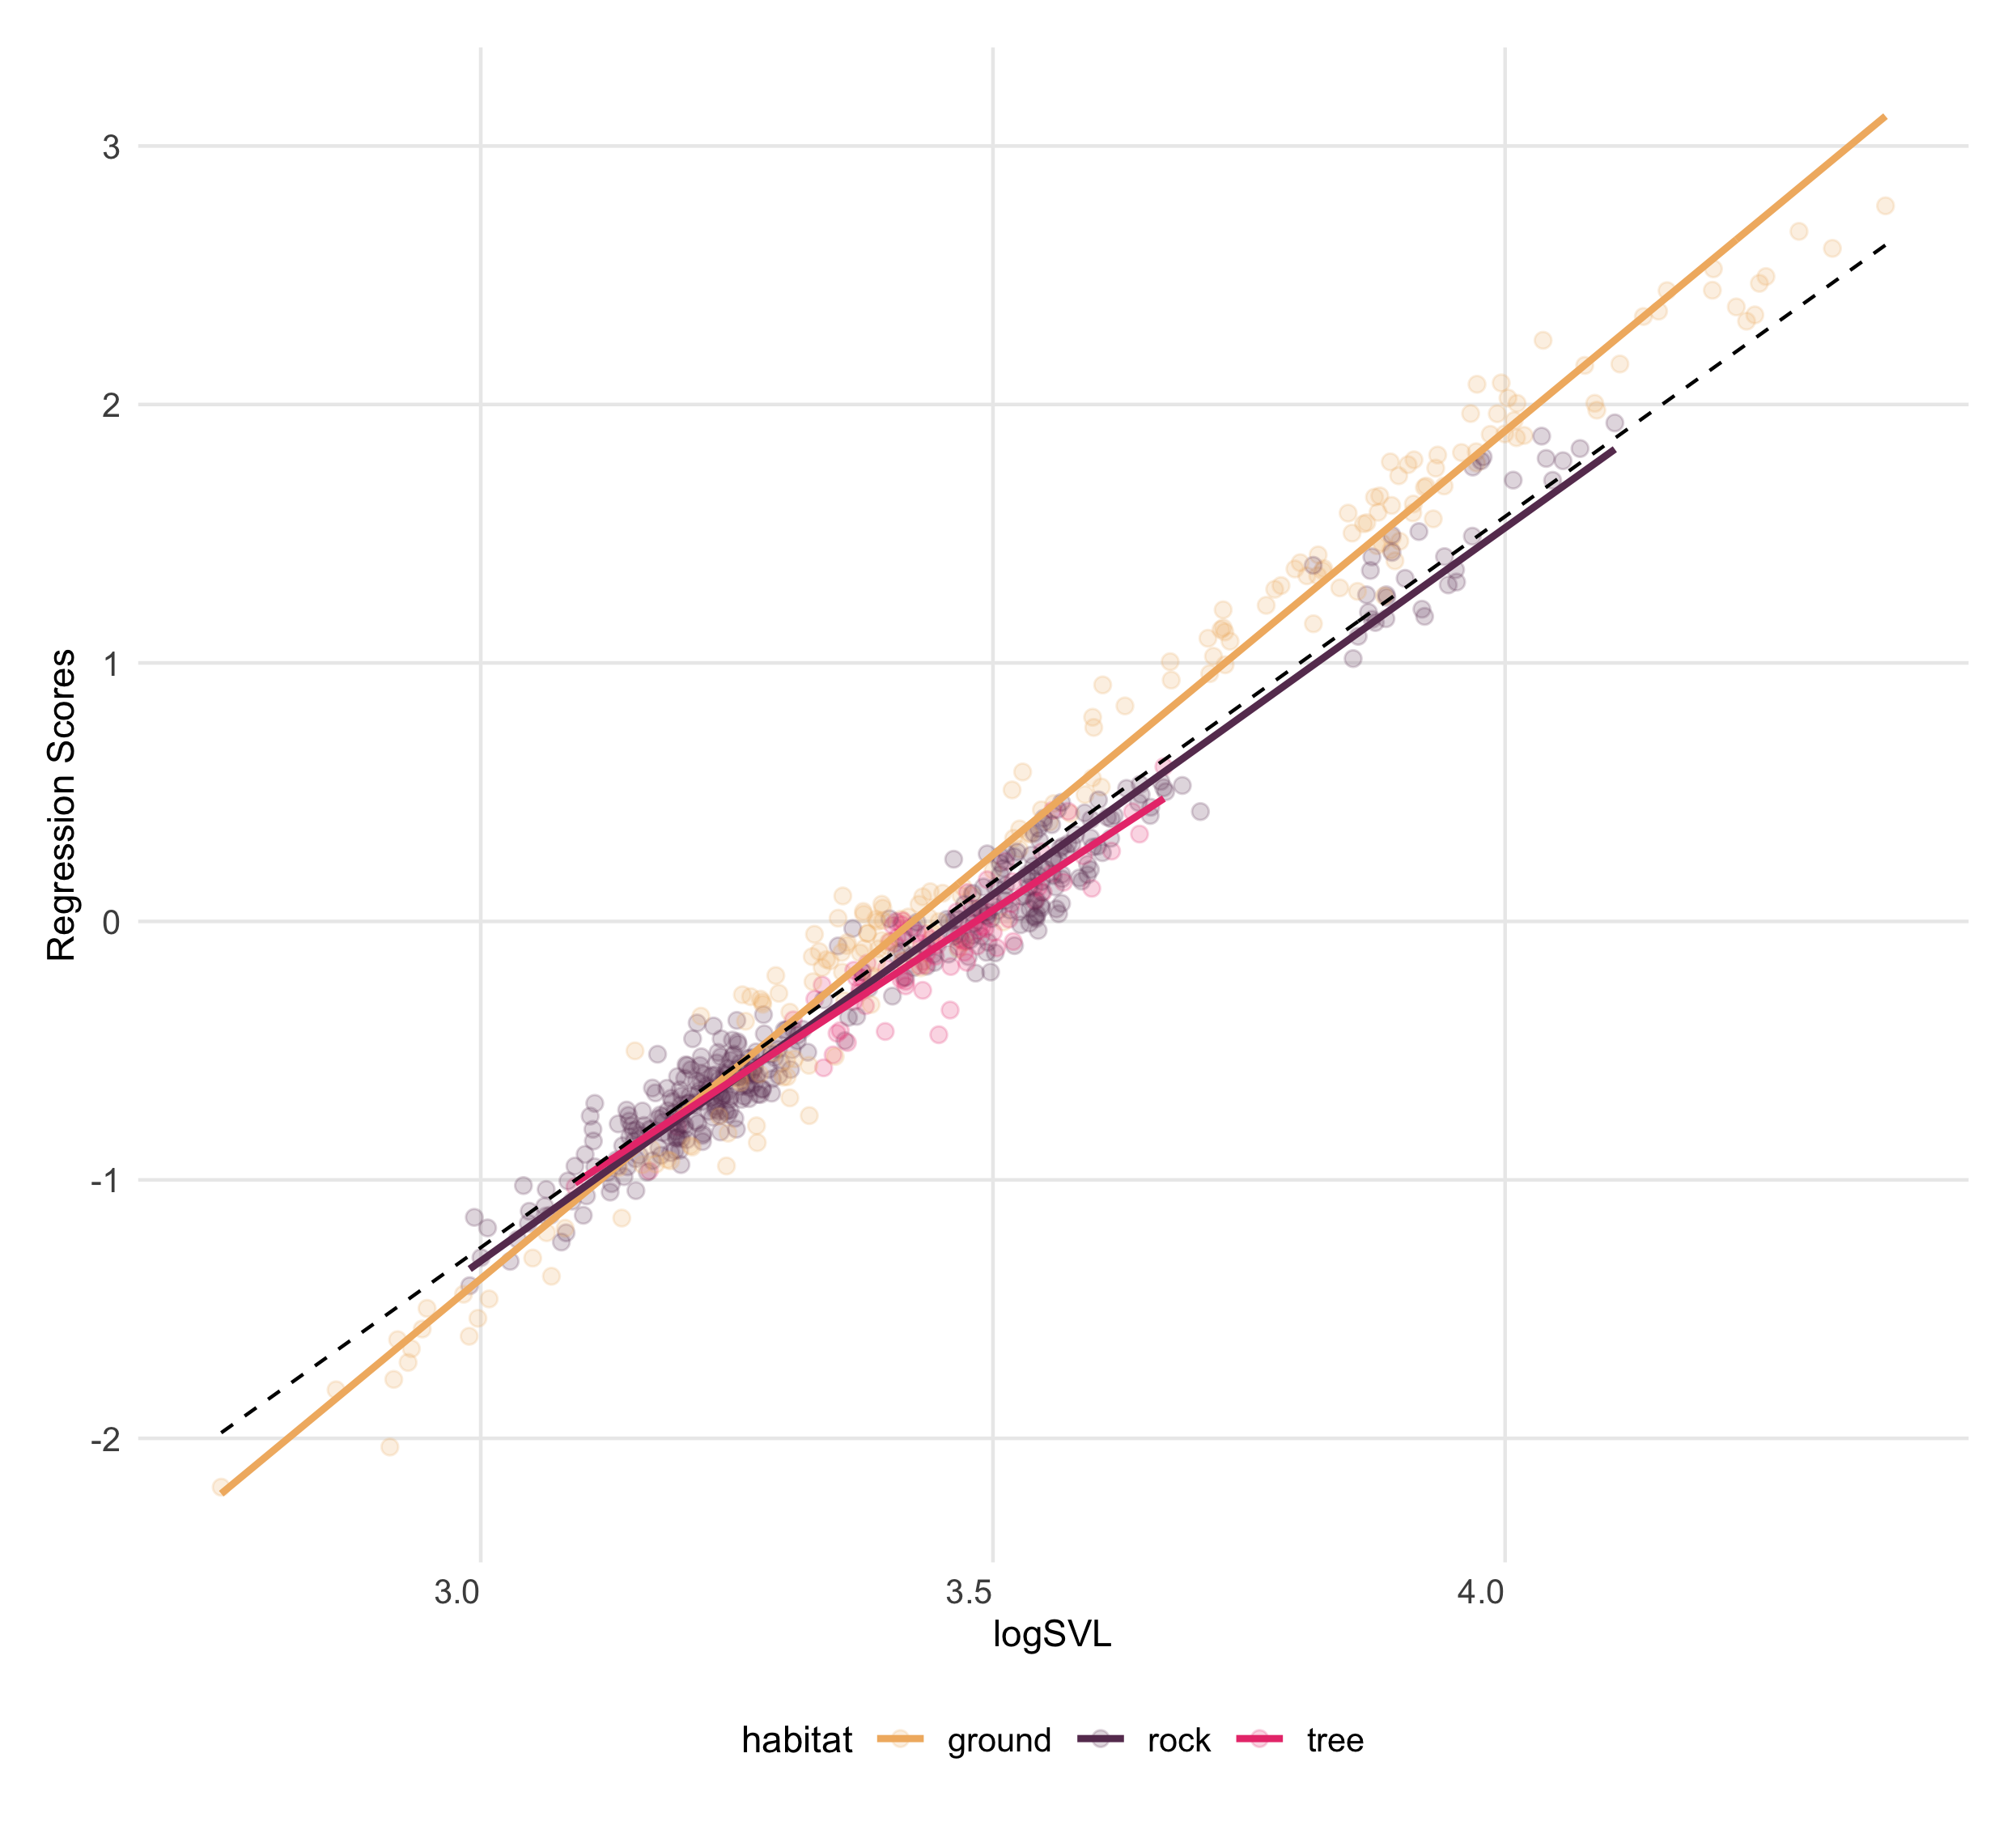
\includegraphics[width=1\linewidth]{Figs/figure_2_ggplot} \caption{Plot of regression scores and predicted lines representing the relationship between linear body measurements and size (SVL). Individuals are colored by habitat use: ground (beige), rock (dark purple), and tree (magenta). Isometric trend represented by the dashed line.}\label{fig:unnamed-chunk-4}
\end{figure}

\newpage

\begin{figure}
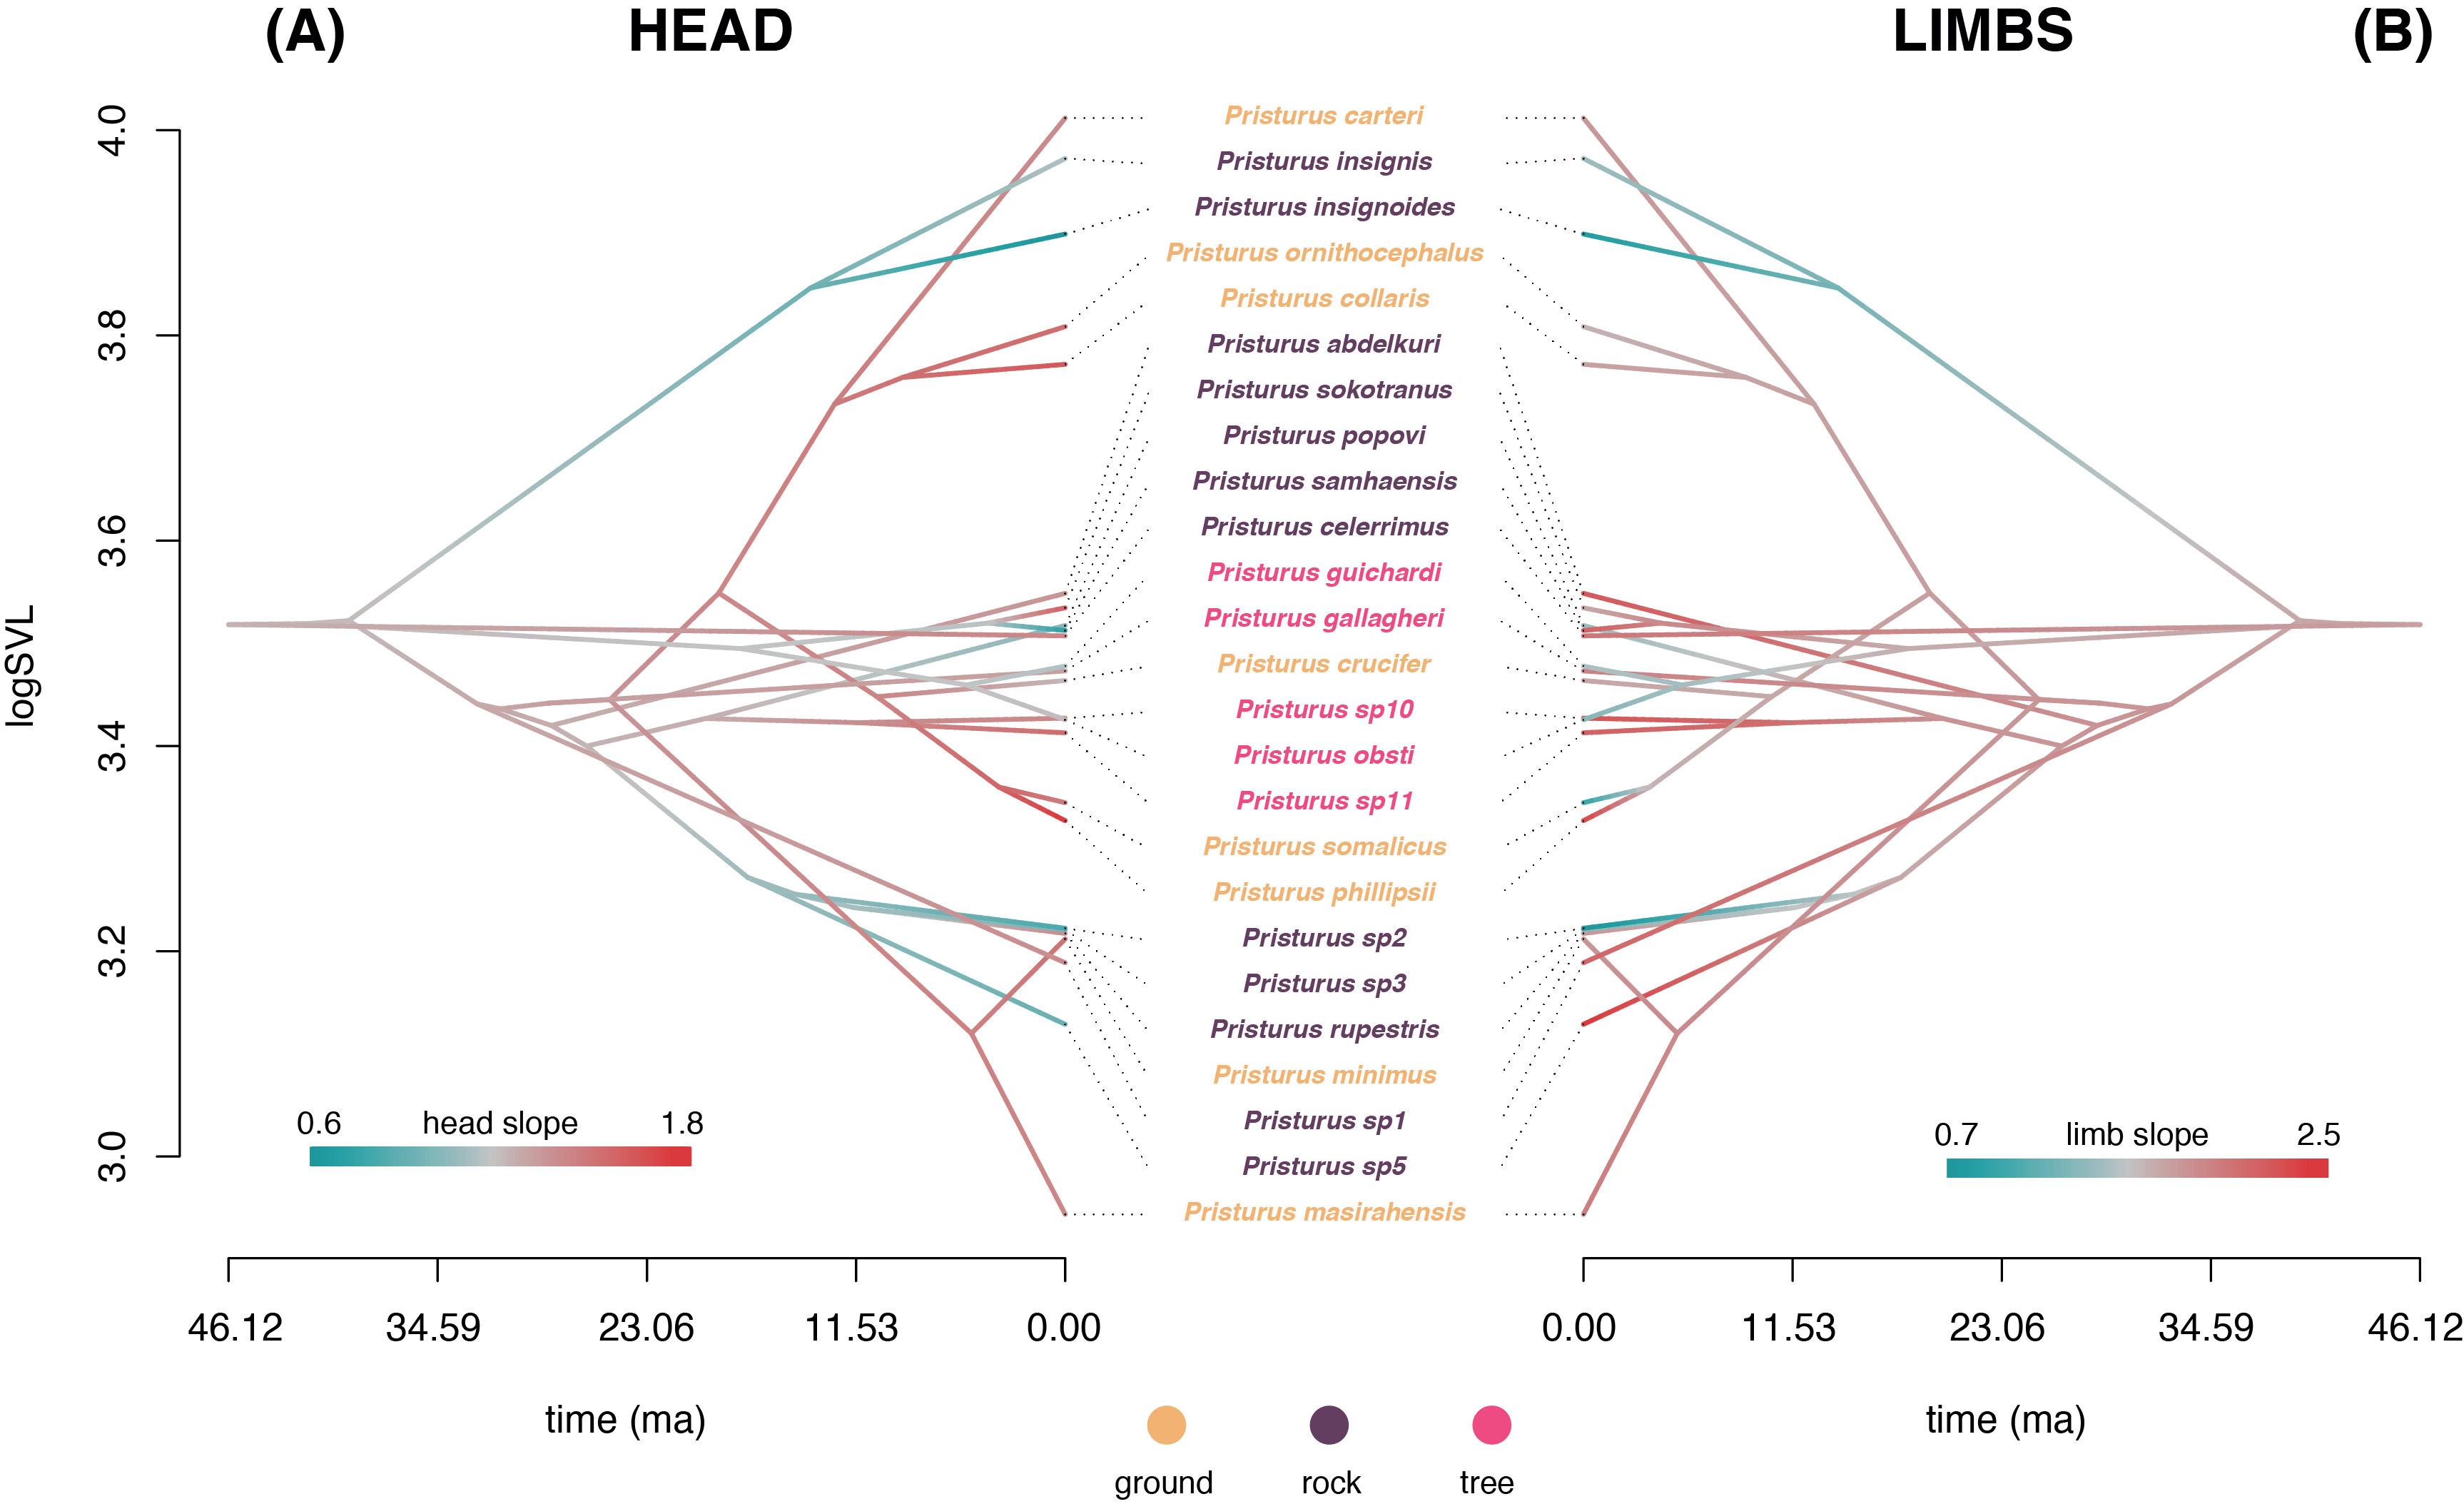
\includegraphics[width=1\linewidth]{Figs/figure_phenograms} \caption{Traitgrams showing the evolution of body size (SVL) through time based on the phylogenetic tree of \textit{Pristurus}. Colors represent an evolutionary mapping of regression slopes describing the relationship of (A) head morphology versus body size, and (B) limb proportions versus body size (see text for descriptions). Species names are colored by habitat use: ground (beige), rock (dark purple), and tree (magenta).}\label{fig:unnamed-chunk-5}
\end{figure}

\newpage

\begin{figure}
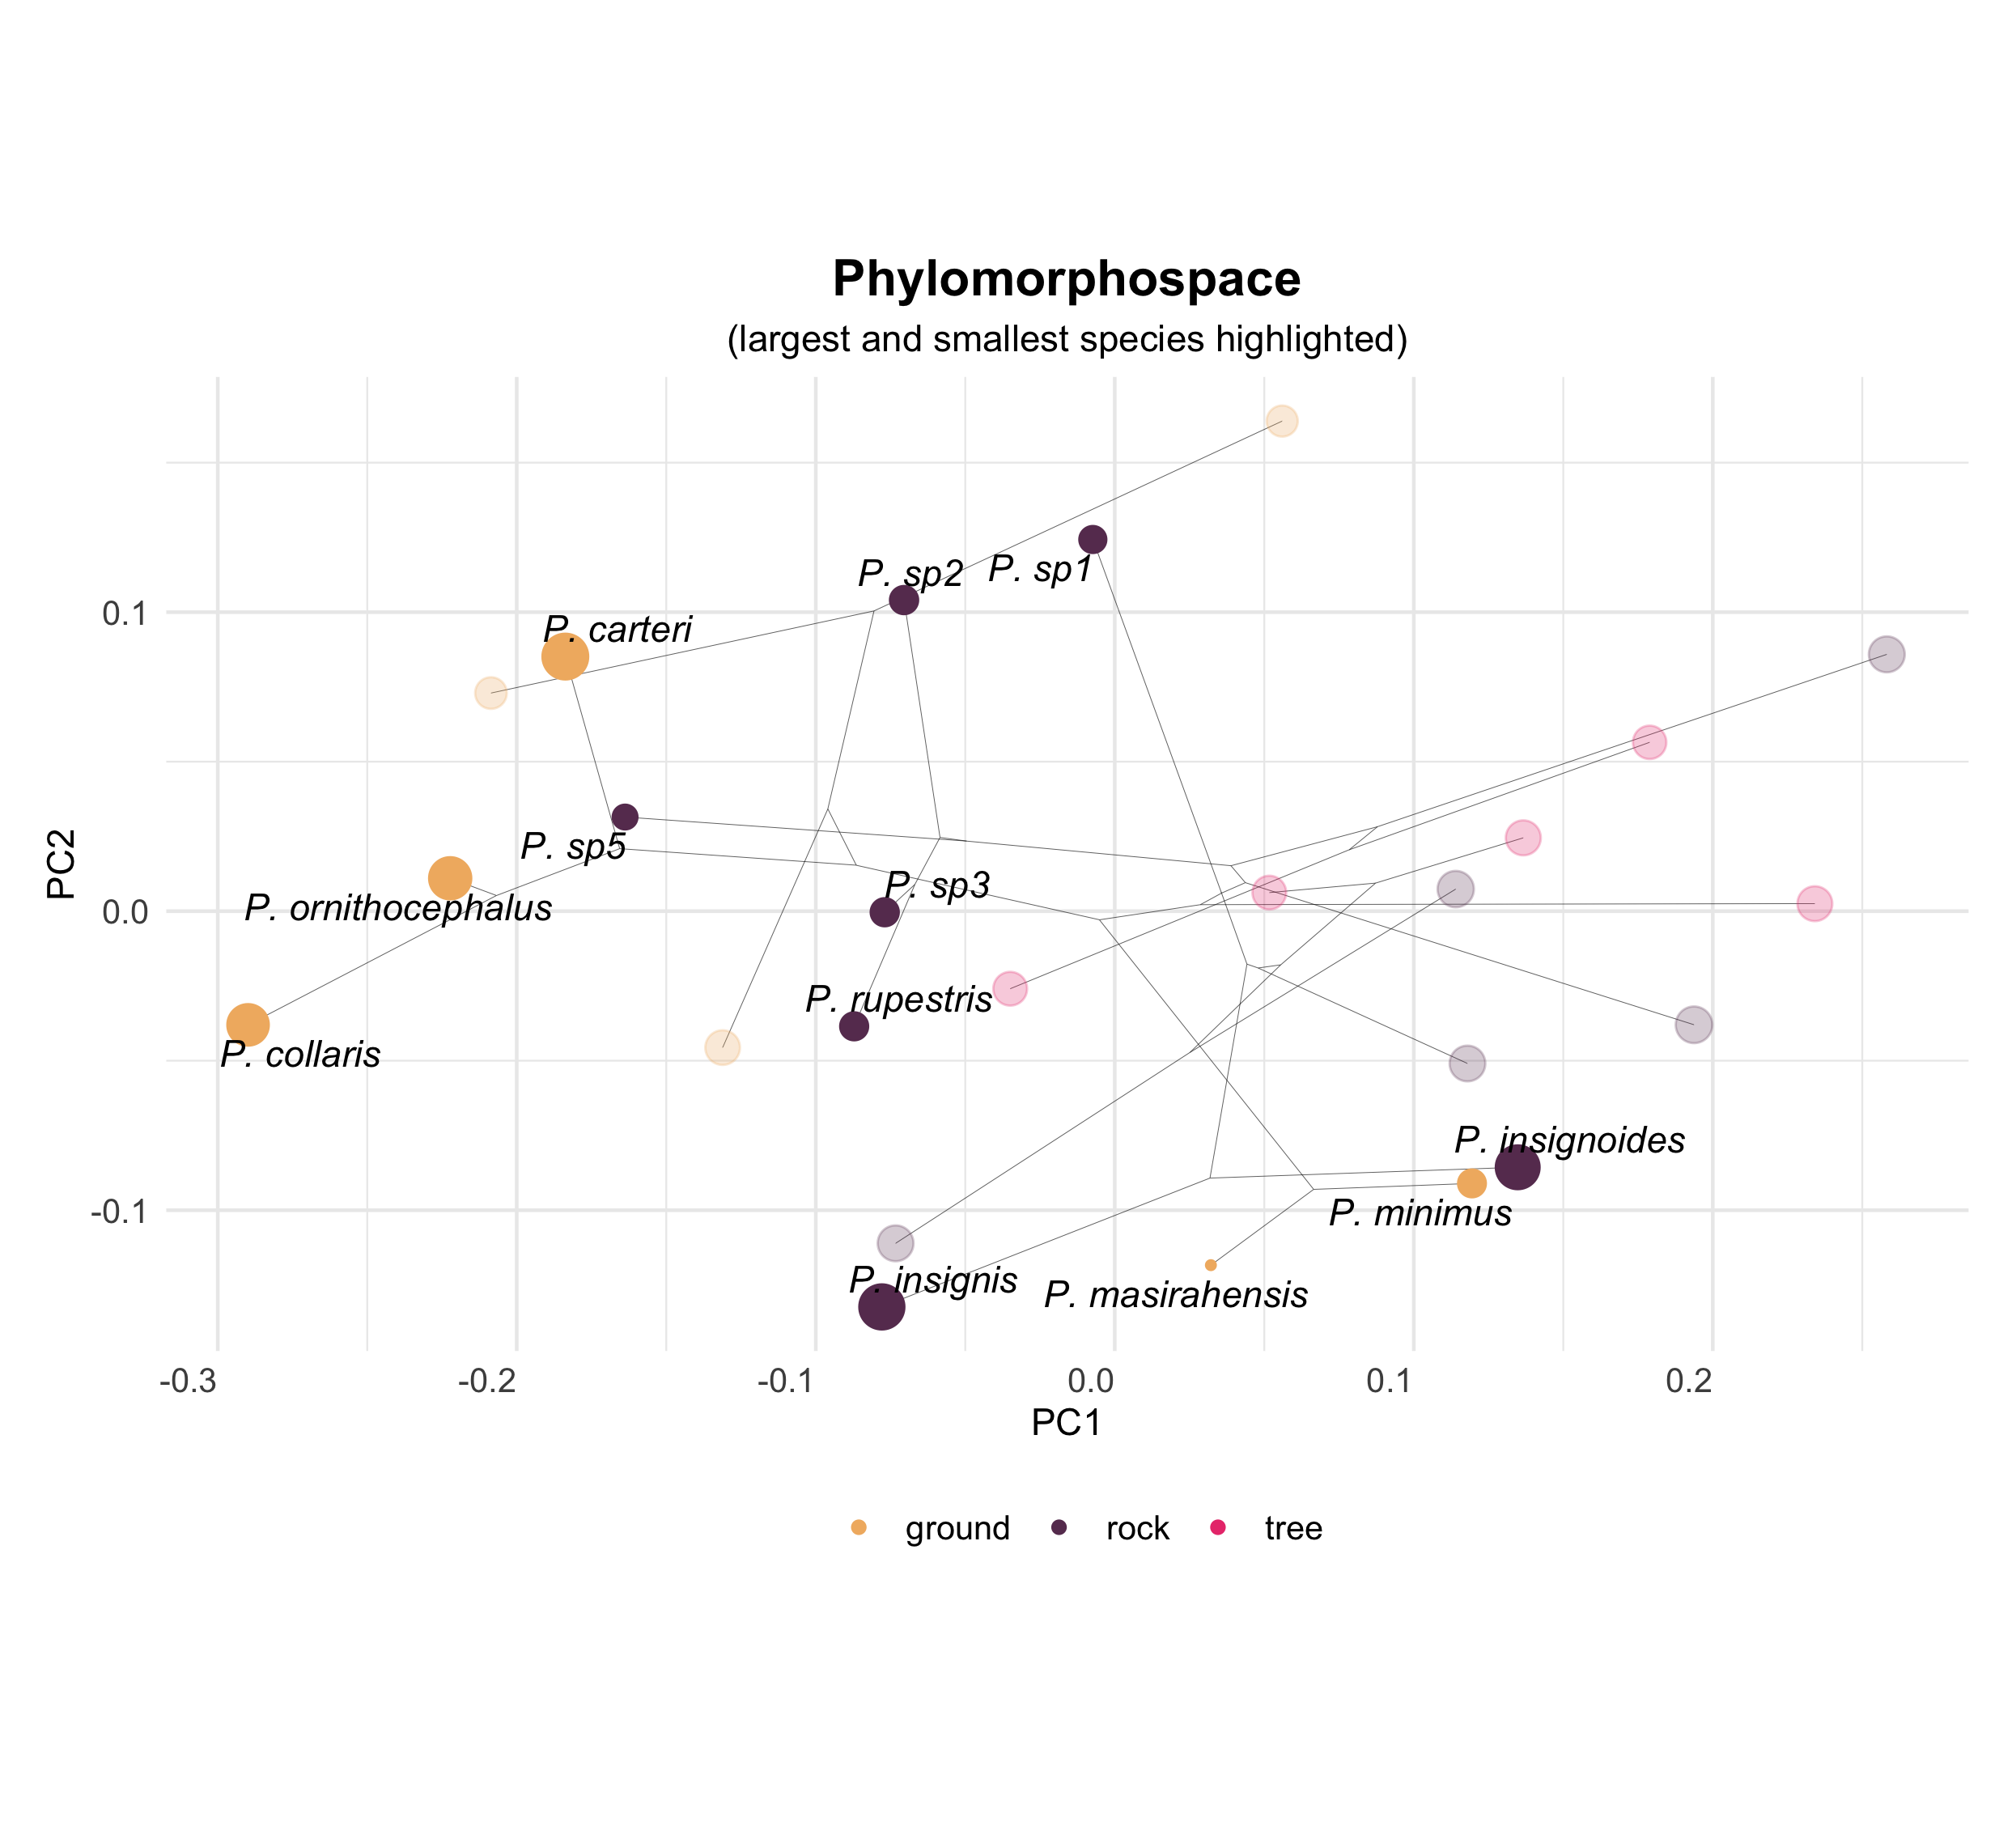
\includegraphics[width=1\linewidth]{Figs/phylomorphospace_large_small} \caption{Phylomorphospace of \textit{Pristurus}, based on residuals from a phylogenetic regression of body measurements on size (SVL). Species means are colored by habitat use: ground (beige), rock (dark purple), and tree (magenta). Large and small rock-dwelling and ground-dwelling are highlighted with darker colors to highlight their differentiation and relative positions in morphospace.}\label{fig:unnamed-chunk-6}
\end{figure}

\end{document}
